\documentclass{article}
\usepackage{titling}
\usepackage[T1]{fontenc}
\usepackage[polish]{babel}
\usepackage[OT4]{fontenc} 
% Margins in document
\usepackage[left=1.5cm, right=1.5cm, top=3cm]{geometry}

% Avoid  colons before tables' empty captions and change caption
\usepackage{caption}
\captionsetup[table]{name=Tab.}
\captionsetup[figure]{name=Rys.}

% Don't know why, it starts from 2
\addtocounter{table}{-1}

% Rename tables' suffix
\renewcommand{\tablename}{Tab.}

% Graphicx setup
\usepackage{graphicx}
\graphicspath{{grafiki/}{../grafiki/}}

% No separator between items
\usepackage{enumitem}
\setlist{nolistsep}

% Pagebreak before every \section
\let\oldsection\section
\renewcommand\section{\clearpage\oldsection}

% Vhistory setup
\usepackage[owncaptions]{vhistory}
\renewcommand{\vhhistoryname}{Historia zmian}
\renewcommand{\vhversionname}{Wersja}
\renewcommand{\vhdatename}{Data}
\renewcommand{\vhauthorname}{Autor(zy)}
\renewcommand{\vhchangename}{Zmiany}

% Bigger padding in tabulars
\usepackage{array}
\setlength\extrarowheight{3pt}

% Itemize in tabulars (avoid big margins with minipage)
\newcommand{\tabbeditemize}[1]{
	\begin{minipage}[t]{0.4\textwidth}
		\begin{itemize}[topsep=0mm,partopsep=0mm,leftmargin=4mm]
			#1
		\end{itemize}
\end{minipage}}

% Code command
\usepackage{xcolor}
\definecolor{light-gray}{gray}{1}
\newcommand{\code}[1]{\colorbox{light-gray}{\texttt{#1}}}

% Modulename command
\newcommand{\modulename}[1]{\textit{#1}}


% DOCUMENT
\title{
	Wizualizacja drzewa stanów algorytmu UCT \\
	\large Plan projektu}

\author{Patryk Fijałkowski \\ Grzegorz Kacprowicz}
\begin{document}
	\begin{titlingpage}
		\maketitle
		\vspace{3cm}
		\begin{abstract}
			Poniższy dokument zawiera ogólny zarys projektu. Aplikacja ma w zamyśle pozwalać na oglądanie i dokładną analizę rozgrywki z komputerem w jedną z dwóch gier planszowych. Istnieje możliwość łatwego rozszerzenia o kolejne gry wpasowujące się w założenia algorytmu UCT. W dokumencie przedstawione są wszystkie moduły aplikacji wraz z pełnionymi funkcjami oraz ich dokładny opis i diagramy UML. Z dokumentu można dowiedzieć się też o zachowaniu poszczególnych komponentów względem siebie oraz jakie opcje są dostępne dla użytkownika. 
		\end{abstract}
	\end{titlingpage}

	\begin{versionhistory}
		\vhEntry{1.0}{3.11.2019}{PF|GK}{stworzenie szkicu dokumentu}
		\vhEntry{1.0}{4.11.2019}{PF|GK}{stworzenie pierwszej wersji dokumentu}
	\end{versionhistory}
	\tableofcontents
	
	\section{Architektura aplikacji}
	Aplikacja będzie podzielona na pięć oddzielnych modułów: \modulename{algorytm}, \modulename{serializacja}, \modulename{wizualizacja}, \modulename{gry}, które będą funkcjonować w obrębie nadrzędnego modułu - \modulename{aplikacji głównej}. Cele każdego z modułów i zadania powierzone im są przedstawione poniżej.
	
	\subsection{Wizualizacja}
	Moduł \modulename{wizualizacja} udostępnia funkcjonalność wizualizacji dostarczonych drzew. Użytkownik będzie miał również możliwość przybliżania, oddalania oraz poruszania się po wizualizacji. Opisana interaktywność ma na celu umożliwić dokładne zbadanie struktury drzewa oraz poszczególnych wartości w interesujących go wierzchołkach. \\
	
	\noindent Dla czytelnych wizualizacji, poczyniliśmy następujące założenia: \\
	
	\begin{enumerate}
		\item Krawędzie drzewa nie mogą się przecinać.
		\item Wierzchołki będą ustawione od góry w rzędach, a przynależność do
		rzędów będzie zależała od odległości wierzchołków od korzenia.
		\item Wierzchołki mają być narysowane możliwie najwęziej.  \\
	\end{enumerate}

	\noindent Aby wyznaczyć układ wierzchołków na płaszczyźnie, spełniając powyższe 3 założenia, skorzystamy z usprawnionego algorytmu Walkera, który działa w czasie liniowym względem liczby wierzchołków. Algorytm, który zaimplementujemy, został opisany w pracy \textit{Improving Walker's Algorithm to Run in Linear Time}\footnote{\modulename{Improving Walker's Algorithm to Run in Linear Time} - Christop Buchheim, Michael Jünger, Sebastian Leipert, Universität zu Köln, Institut für Informatik}.
	
	\subsection{Algorytm}
	Moduł \modulename{Algorytm} jest implementacją algorytmu Monte Carlo Tree Search, korzystającą z wariantu UCT. Odpowiedzialnością tego modułu jest wyznaczanie kolejnego ruchu na podstawie dostarczonego stanu gry. Opisywany moduł będzie odpowiadał za iteracyjne tworzenie drzewa stanów i przeszukiwanie go w celu wyznaczenia najbardziej korzystnego ruchu. Użytkownik będzie miał możliwość zmiany liczby iteracji algorytmu albo ograniczenie czasowe jego działania. \\
	
	\noindent Aby gra była poprawnie obsłużona przez moduł \modulename{algorytm}, musi spełniać następujące założenia: \\
		
	\begin{enumerate}
		\item Rozgrywka jest prowadzona naprzemiennie przez dwóch graczy.
		\item Każdy ruch ma jednoznaczny wpływ na dalszą rozgrywkę (rozgrywka jest deterministyczna).
		\item Każdy z graczy ma dostęp do pełnej informacji o aktualnym stanie gry. \\
	\end{enumerate} 
	
	\noindent Rozdział trzeci zawiera dokładniejszy opis funkcjonalności, które należy zapewnić, by moduł \modulename{Algorytm} mógł wyznaczać kolejne ruchy danej gry.
	
%	\noindent Pseudokod algorytmu jest opisany w listingu \ref{...}.
%	\lstlisting{
%	iterations_counter = 0;
%	tree = initialize_tree();
%	while (iterations_counter < max_iterations_counter)
%	{
%	  node = selection(tree.root);
%	  expansion(node);
%	  playout_result = simulation(node);
%	  backpropagation(node, playout_result); //TODO: dorzuc do UMLa
%	  
%	  iterations_counter++;
%	}
%	best_state = select_best_child(tree.root) //TODO: niedokladne
%	return best_state;
%	}
	
	
	\subsection{Gry}
	Aplikacja będzie udostępniała 2 gry planszowe umożliwiające zademonstrowanie efektywności wizualizacji oraz algorytmu. Obie gry będą umożliwiały różne tryby rozgrywki: \\
	
	\begin{itemize}
		\item \textbf{Człowiek kontra maszyna:} decyzje jednego z graczy są podejmowane przez użytkownika, natomiast drugi gracz podejmuje decyzje najoptymalniejsze z punktu widzenia algorytmu UCT.
		\item \textbf{Maszyna kontra maszyna:} decyzje obojga graczy są podejmowane przez algorytm. \\ 
	\end{itemize}
	
	\clearpage
	
	\subsection{Serializacja}
	\modulename{Serializacja} jest modułem odpowiadającym za zapisywanie drzew do plików formacie binarnym lub csv. Oba schematy są rekurencyjne, bo taka jest również struktura generowanych przez aplikację drzew. To oznacza, że w celu zapisania całego drzewa, wystarczy zserializować jego korzeń.\\
	
	\noindent \textbf{\large Serializacja binarna} \\
	W serializacji binarnej przyjmujemy opisany niżej schemat.\\

	\begin{itemize}
		\item \textbf{liczba całkowita} - wartość liczby zakodowanej w U2 na 4 bajtach. Bajty liczby w kolejności little endian.
		\item \textbf{napis}:
		\begin{itemize}
			\item liczba bajtów w napisie \textit{(liczba całkowita)},
			\item zawartość napisu kodowana w UTF8.
		\end{itemize}
		\item \textbf{liczba zmiennoprzecinkowa} - wartość liczby zakodowanej w IEEE754 na 64 bitach w kolejności little endian.
		\item \textbf{wierzchołek:}
		\begin{itemize}
			\item nazwa stanu \textit{(napis)},
			\item $m$ - liczba węzłów potomnych \textit{(liczba całkowita)},
			\item $m$ powtórzeń następującego bytu:
			\begin{itemize}
				\item nazwa ruchu \textit{(napis)},
				\item licznik odwiedzin \textit{(liczba całkowita)},
				\item dodatkowy licznik odwiedzin \textit{(liczba całkowita)},
				\item średnia wypłata \textit{(liczba zmiennoprzecinkowa)},
				\item węzeł potomny \textit{(wierzchołek)}. \\
			\end{itemize}
		\end{itemize}
	\end{itemize}
	
	
	\noindent \textbf{\large Serializacja do plików csv} \\
	W serializacji do plików csv przyjmujemy, że każdy kolejny wiersz odpowiada kolejnemu wierzchołkowi drzewa, a kolejne wartości opisujące wierzchołek oddzielamy przecinkami. Ostatnią wartością jest liczba wierzchołków potomnych. Jeśli wierzchołek $v$ ma $k$ potomków, to pod wierszem opisującym wierzchołek $v$ będzie $k$ wierszy opisujących jego potomków. Każdy wierzchołek serializujemy do wiersza postaci:
	\begin{center}
		\textbf{R, O, O2, W, S, D}
	\end{center}
	Oznaczenia:
	\begin{itemize}
		\item R - nazwa ruchu,
		\item O - licznik odwiedzin,
		\item O2 - dodatkowy licznik odwiedzin,
		\item W - średnia wypłata algorytmu za ruch,
		\item S - nawa stanu,
		\item D - liczba wierzchołków potomnych.
	\end{itemize}

	\subsection{Aplikacja główna}
	\modulename{Aplikacja główna} jest modułem łączącym wszystkie pozostałe. Ten moduł skupia się na zaprezentowaniu funkcjonalności wszystkich modułów w formie aplikacji okienkowej. Obszerny opis projektu aplikacji okienkowej znajduje się w rozdziale czwartym.
	
	\section{Główne komponenty aplikacji}
	\subsection{Diagram klas głównych komponentów}
	
	\noindent Rysunek \ref{rys:umldiagrammain} ukazuje diagram klas najważniejszych komponentów związanych z modułami \modulename{Algorytm}, \modulename{Wizualizacja} i \modulename{Serializacja}.
	
	\begin{figure}[h]
		\centering
		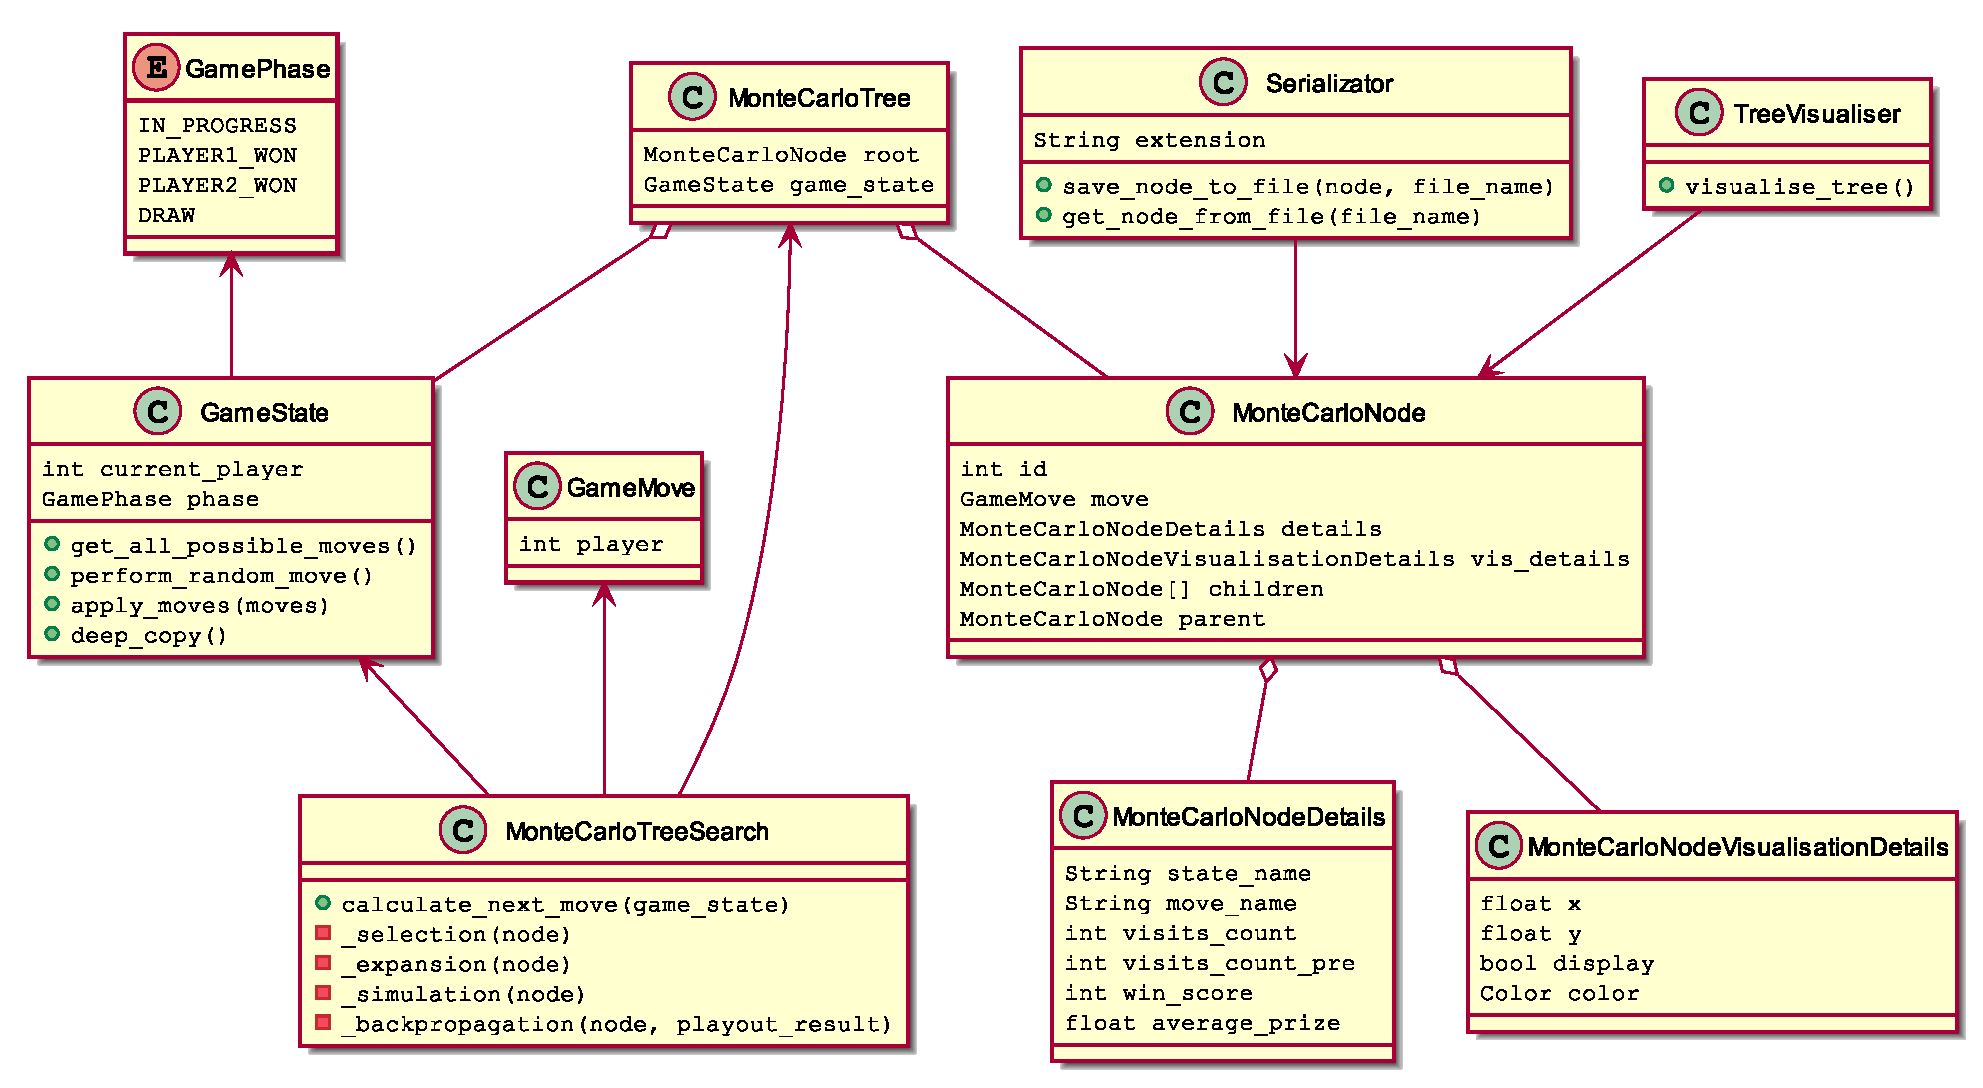
\includegraphics[width=0.9\textwidth]{umldiagram}
		\caption{Diagram klas głównych komponentów}
		\label{rys:umldiagrammain}
	\end{figure}
	 \noindent Opis wierzchołka drzewa jest częścią wspólną dla każdego z tych modułów. Zgodnie z diagramem, klasy \code{MonteCarloTreeSearch}, \code{TreeVisualiser} oraz \code{BaseSerializator} są pośrednio lub bezpośrednie zależne od klasy \code{MonteCarloNode}. \\
	
	\noindent Metoda \code{calculate\textunderscore next\textunderscore move} klasy \code{MonteCarloTreeSearch} odpowiada za wykonanie kolejnych iteracji algorytmu. Ruch oraz stan analizowanej gry są opisane odpowiednio przez klasy \code{BaseGameMove} i \code{BaseGameState}. Implementacja metod tych klas daje możliwość łatwego rozszerzenia aplikacji o inne gry. Istotny z punktu widzenia konstrukcji drzewa jest stan rozgrywki, który opisują pola typu wyliczeniowego \code{GamePhase}. \\
	
	\noindent \code{TreeVisualiser} jest głównym komponentem modułu \modulename{Wizualizacja}. Jego odpowiedzialnością jest wyznaczenie układu wierzchołków drzewa na płaszczyźnie oraz wyświetlenie wygenerowanej wizualizacji. Szczegóły związane z rysowaniem każdego wierzchołka zawarte są w \code{MonteCarloVisualisationDetails}.
	
	\clearpage
	\subsection{Diagram stanów aplikacji}
	\noindent Rysunek \ref{rys:statediagram} ukazuje diagram stanów aplikacji w przypadku rozgrywki w trybie \modulename{człowiek kontra maszyna}. 
	\begin{figure}[h]
		\centering
		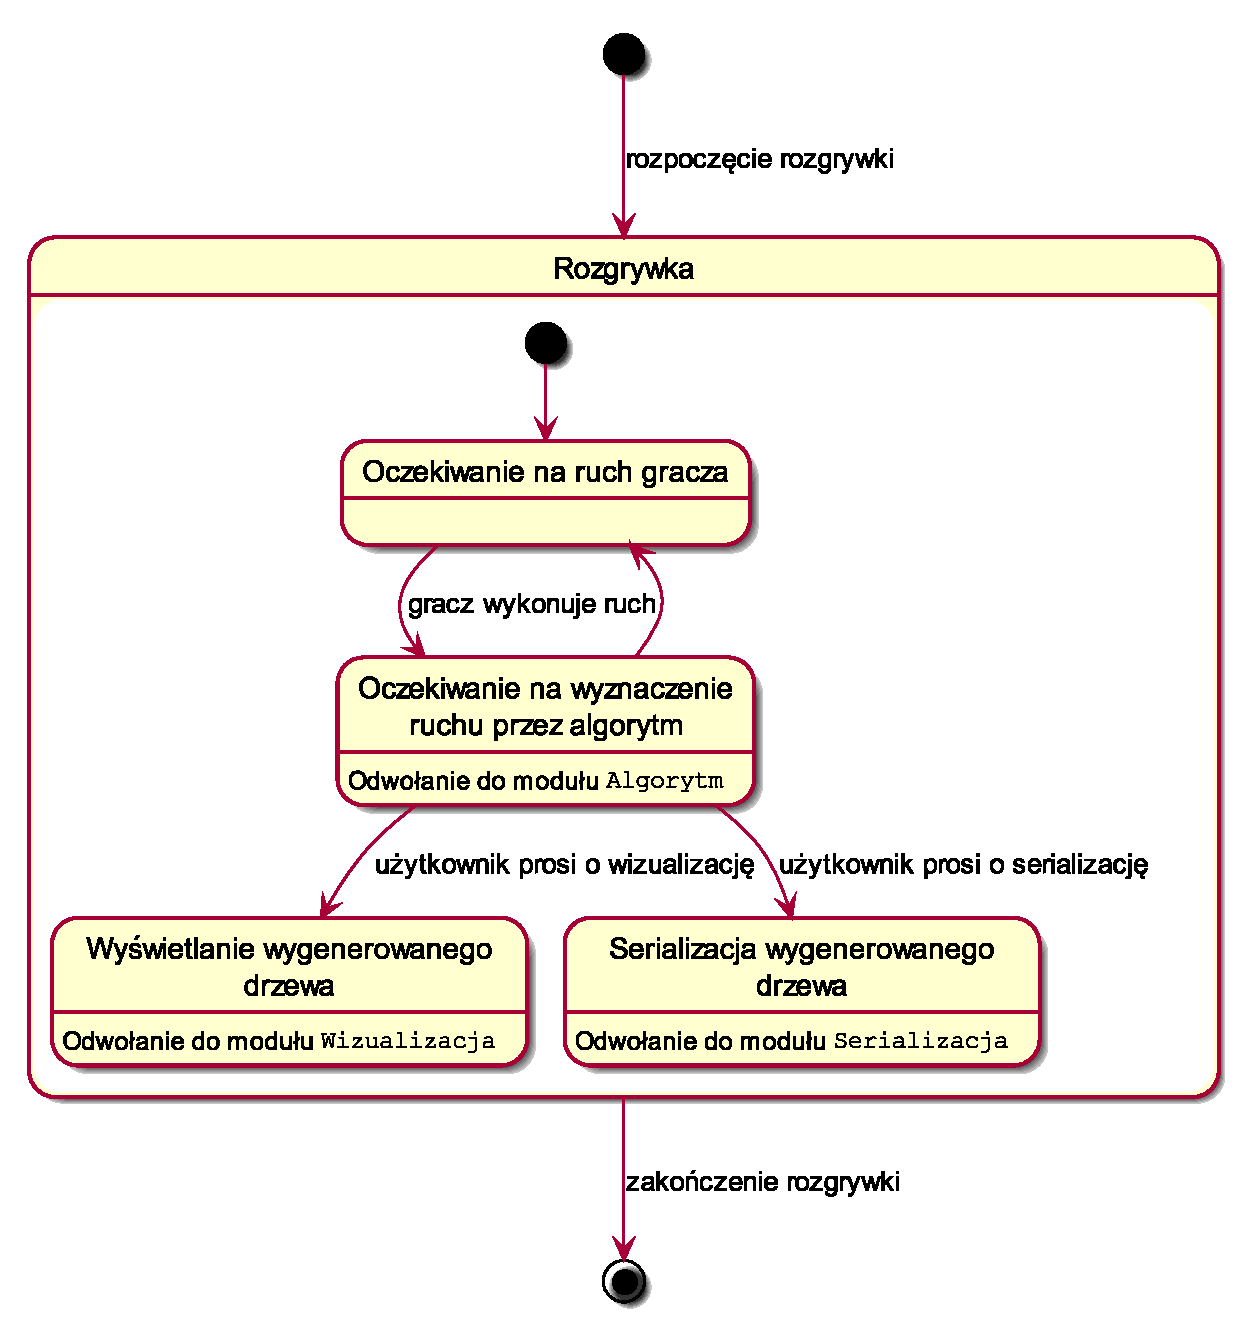
\includegraphics[width=0.7\textwidth]{statediagram}
		\caption{Diagram stanów aplikacji}
		\label{rys:statediagram}
	\end{figure}

	\noindent Zgodnie z diagramem, aplikacja po rozpoczęciu rozgrywki przechodzi do obszernego stanu \modulename{Rozgrywka}, zawierającego cztery wewnętrzne stany. Będac w stanie \modulename{Rozgrywka}, aplikacja może potencjalnie korzystać z każdego modułu aplikacji. \\
	
	\noindent Istotna z punktu widzenia użytkownika jest możliwość serializowania wygenerowanego drzewa lub jego wizualizacja zaraz po ruchu wyznaczonym przez algorytm, co powoduje przejście aplikacji odpowiednio w stany \modulename{Serializacja wygenerowanego drzewa} oraz \modulename{Wyświetlanie wygenerowanego drzewa}.
	\clearpage
	
	\subsection{Diagram sekwencji rozgrywki}
	Rysunek \ref{rys:sequencegame} ukazuje diagram sekwencji rozgrywki w trybie \modulename{człowiek kontra maszyna}.
	\begin{figure}[h]
		\centering
		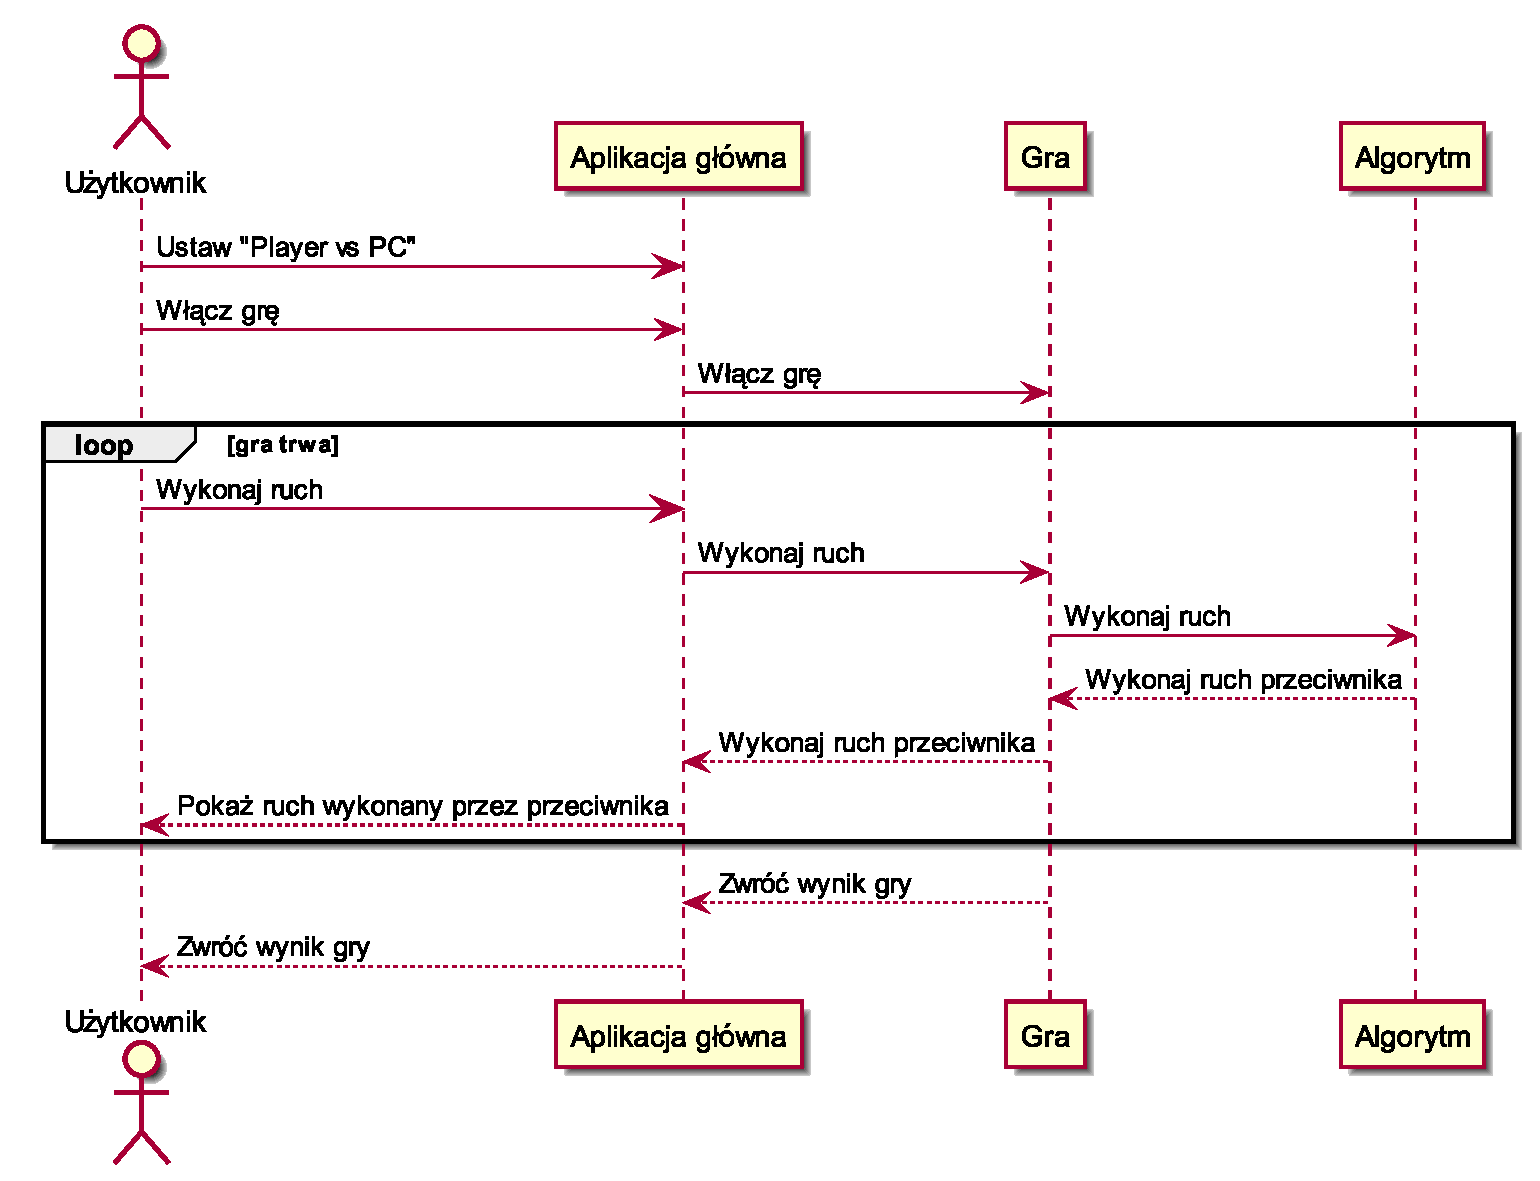
\includegraphics[width=0.8\textwidth]{play_with_pc_sequence}
		\caption{Diagram sekwencji rozgrywki}
		\label{rys:sequencegame}
	\end{figure}

	\noindent Istotne jest, jak w tej sytuacji komunikują się ze sobą moduły \modulename{Aplikacja główna}, \modulename{Gra} i \modulename{Algorytm}. Zgodnie z założeniami, \modulename{Aplikacja główna} jest interfejsem użytkownika do korzystania z pozostałych modułów.\\
	
	\noindent Diagram ukazuje również, że w tym trybie każdy ruch gracza jest ściśle związany z odpowiedzią od modułu \modulename{Algorytm}, który pobiera stan rozgrywki z modułu \modulename{Gra}.
	
	\clearpage
	\subsection{Diagram sekwencji eksportu drzewa}
	Rysunek \ref{rys:sequenceserialize} przedstawia proces współpracy różnych komponentów aplikacji w celu wyeksportowania wygenerowanego przez algorytm drzewa.
	\begin{figure}[h]
		\centering
		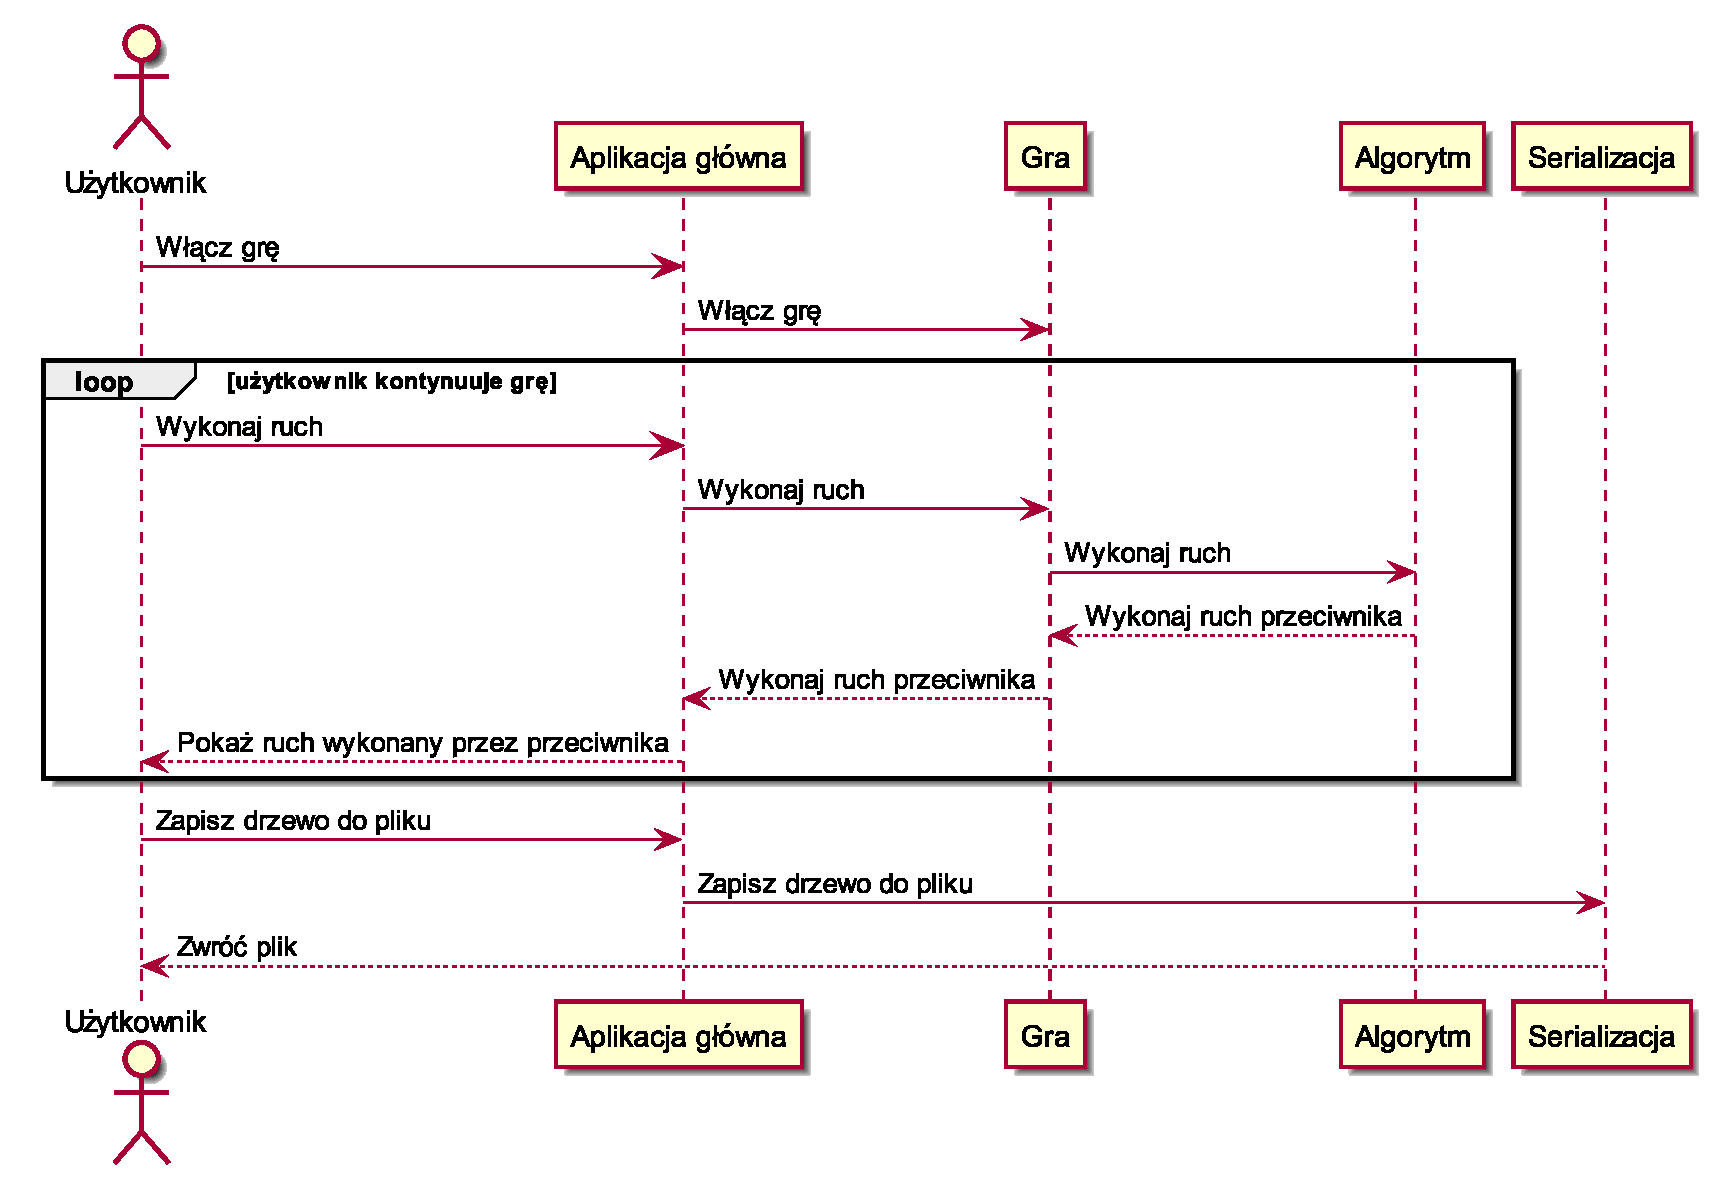
\includegraphics[width=0.8\textwidth]{serialize_sequence}
		\caption{Diagram sekwencji eksportu drzewa}
		\label{rys:sequenceserialize}
	\end{figure}

	\noindent Istotną cechą zaprojektowanego rozwiązania jest to, że gracz może to zrobić w dowolnym momencie rozgrywki (po każdym ruchu przeciwnika). Jest to diagram dla ustawienia \modulename{człowiek kontra maszyna}, jednak w przypadku \modulename{maszyna kontra maszyna} istnieje taka sama funkcjonalność i diagram byłby analogiczny.
	
	\clearpage
	\subsection{Diagram sekwencji wizualizacji}
	Diagram \ref{rys:sequencevisualise} przedstawia proces uruchamiania wizualizacji drzewa przez użytkownika jako współpracę poszczególnych komponentów aplikacji.
	\begin{figure}[h]
		\centering
		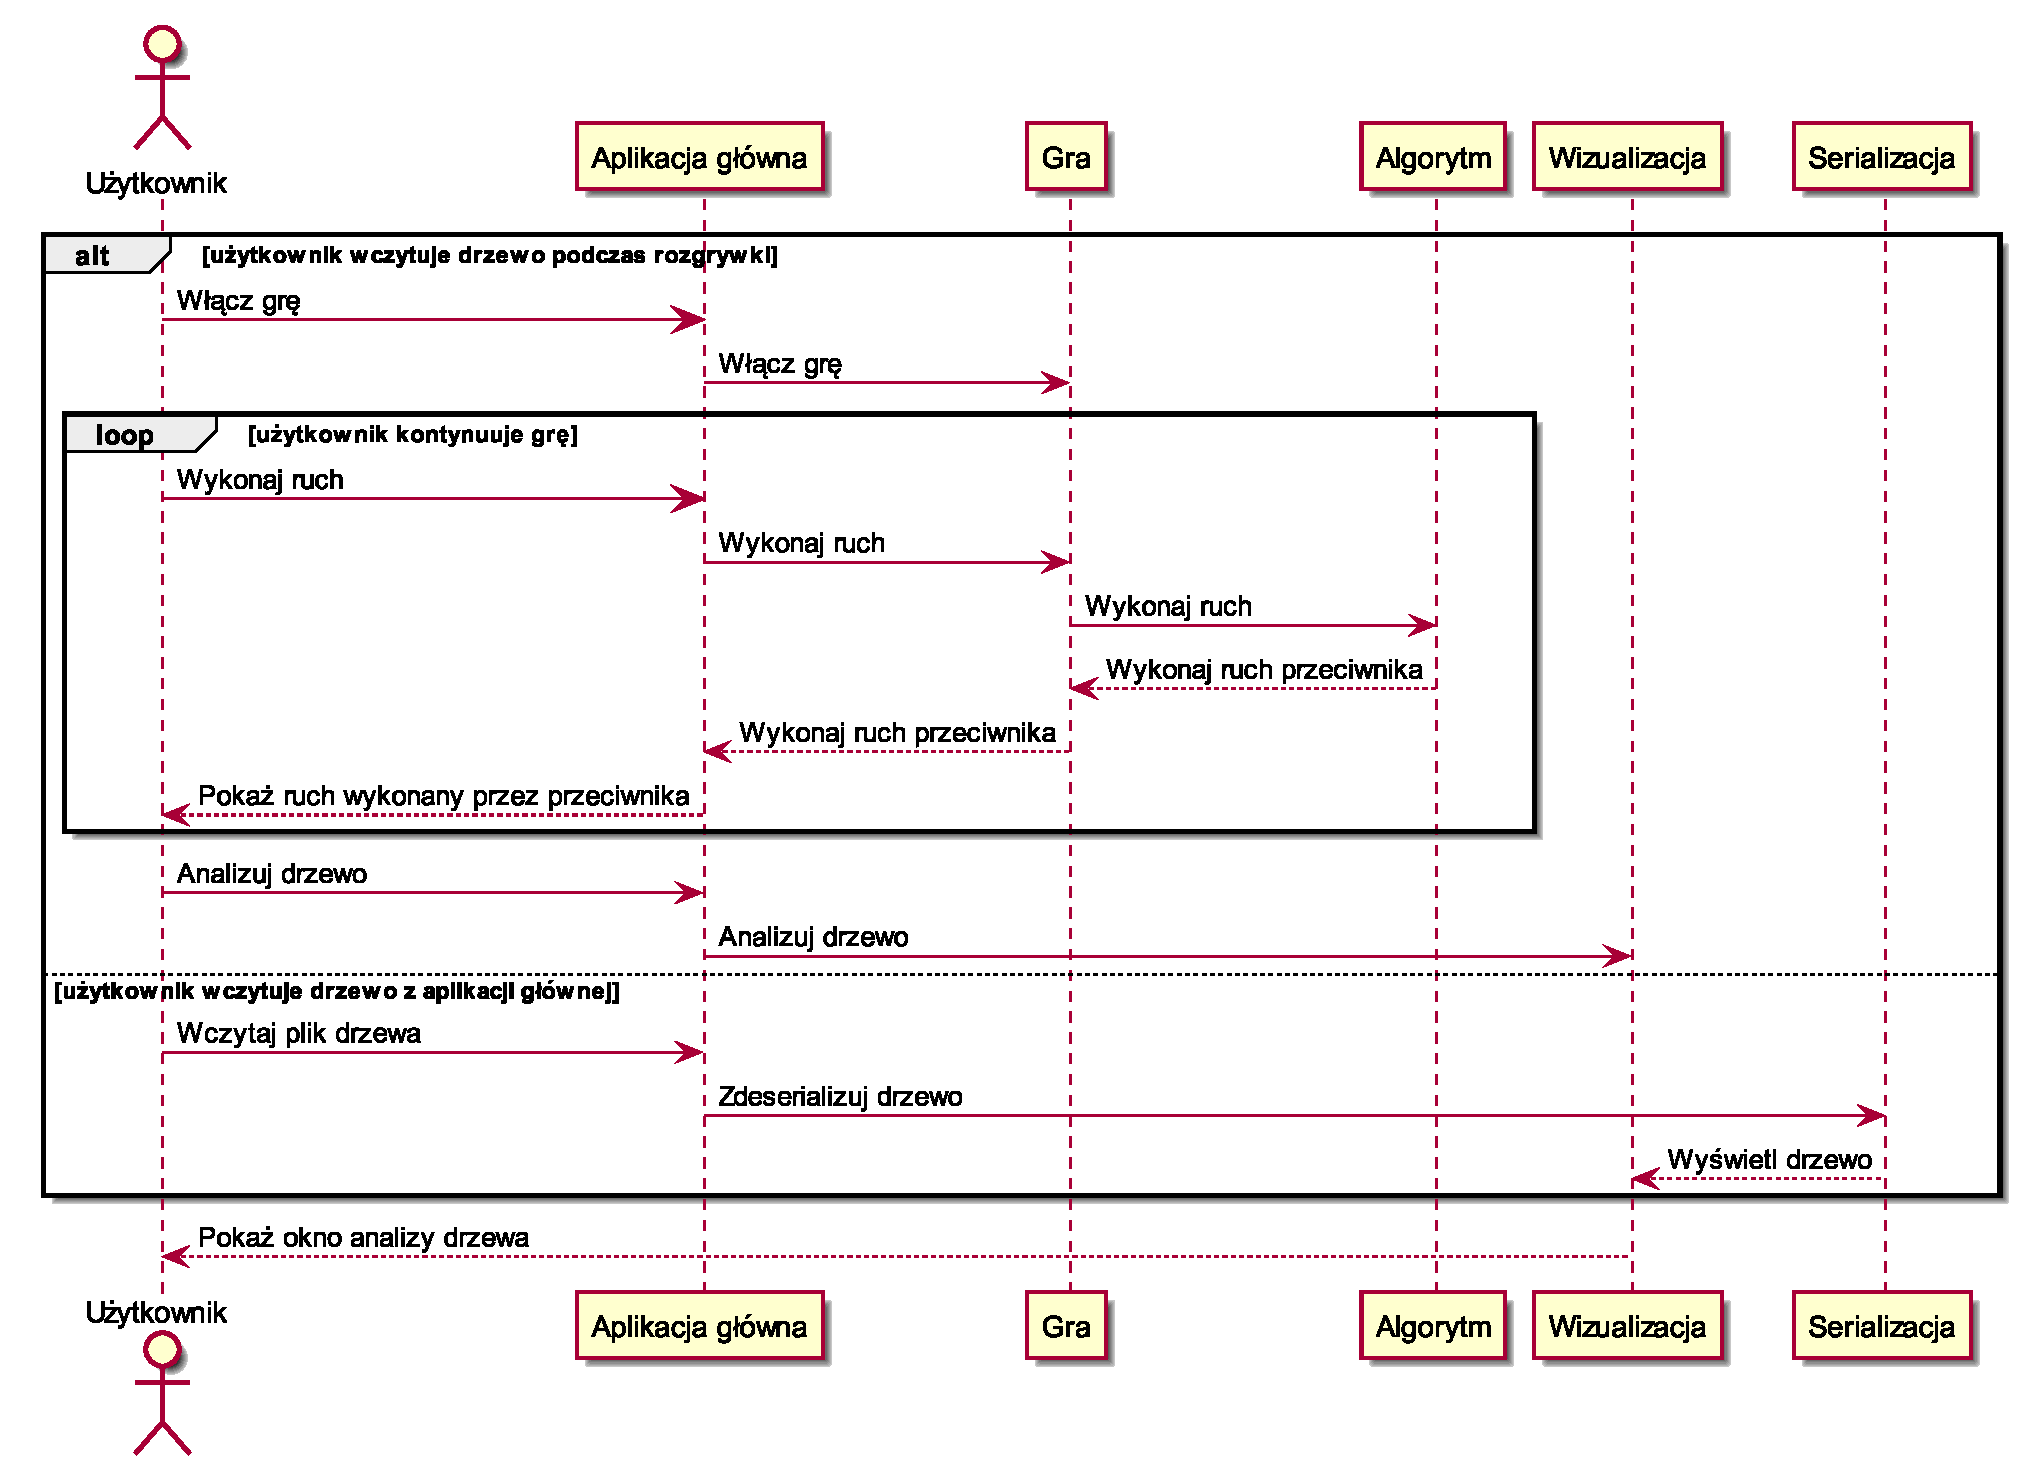
\includegraphics[width=0.8\textwidth]{visualization_sequence}
		\caption{Diagram sekwencji wizualizacji}
		\label{rys:sequencevisualise}
	\end{figure}

	\noindent Ważne jest, że użytkownik może uruchomić wizualizację z poziomu rozgrywki, tuż po wygenerowaniu nowego drzewa przez algorytm lub już na etapie menu głównego. Ten drugi sposób wymaga wcześniejszego wczytania drzewa z pliku i odpowiednio jego deserializację w celu wyświetlenia.
	
	\section{Interfejs użytkownika}
	Graficzny interfejs użytkownika składać się będzie z trzech głównych okien, a logika jego działania będzie w całości zawarta w module \modulename{Aplikacja główna}. Zadaniem graficznego interfejsu jest umożliwienie uruchomienia poszczególnych modułów użytkownikom końcowym.
	
	\subsection{Menu główne}
	Ukazane na rysunku \ref{rys:main_menu} menu główne będzie głównym oknem aplikacji i będzie to pierwsza rzecz, którą zobaczy użytkownik po uruchomieniu programu.
	\begin{figure}[h!]
		\centering
		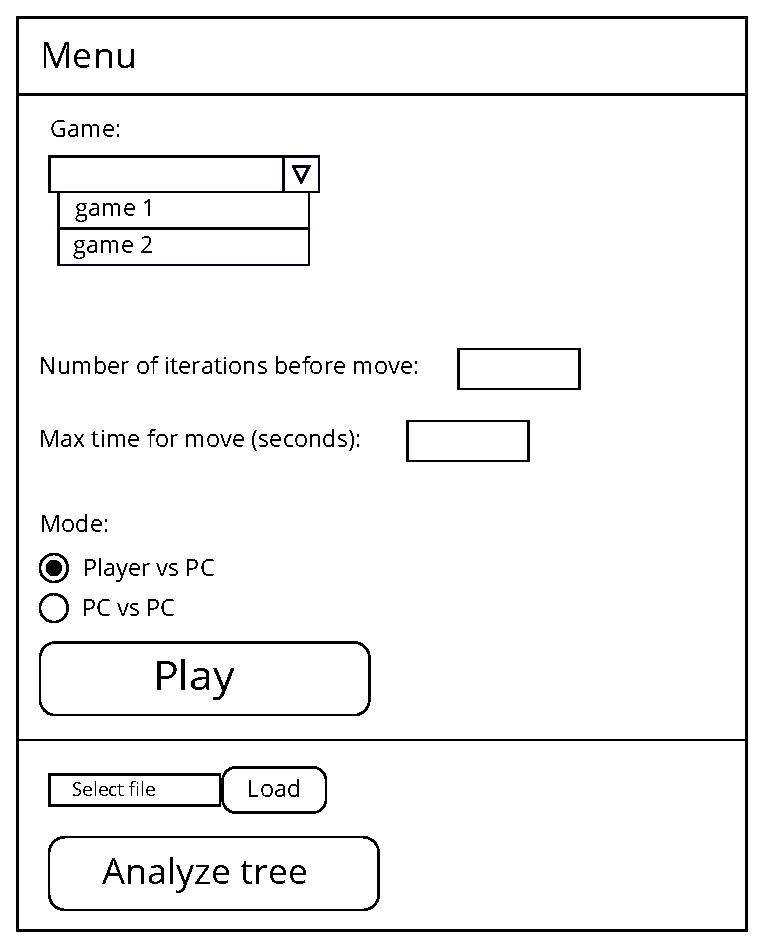
\includegraphics[width=0.4\textwidth]{menu-eps}
		\caption{Okno menu głównego}
		\label{rys:main_menu}
	\end{figure}

	\noindent Dwa moduły, do których można przejść z tego okna, to rozgrywka i analiza drzewa.	Żeby rozegrać grę, należy nacisnąć na przycisk \textit{Play}. Powyżej tego przycisku znajdować się będzie szereg opcji, który pozwoli użytkownikowi ustawić parametry gry dostosowane do jego preferencji, w tym między innymi:\\
	
	\begin{itemize}
		\item wybór gry - rozwijalna lista, w której znajdować się będą zaimplementowane gry (nasz projekt przewiduje dwa tytuły),
		\item liczba iteracji (rozgrywek), jaką komputer będzie wykonywał przed wykonaniem ruchu,
		\item maksymalny czas na wykonanie ruchu - czas, po którym komputer będzie przerywał obliczenia i wykona ruch,
		\item tryb rozgrywki:
		\subitem - człowiek kontra człowiek,
		\subitem - człowiek kontra maszyna,
		\subitem - maszyna kontra maszyna,\\
	\end{itemize}

	\noindent Analiza drzewa będzie dostępna po naciśnięciu przycisku \textit{Analyze tree} i uprzedniego wczytania pliku z zserializowanym drzewem (.tree, .csv).
	
	\clearpage
	\subsection{Analiza drzewa}
	W oknie ukazanym na rysunku \ref{rys:analyze_tree} będziemy mogli oglądać wczytane lub wygenerowane drzewo. 
	\begin{figure}[h!]
		\centering
		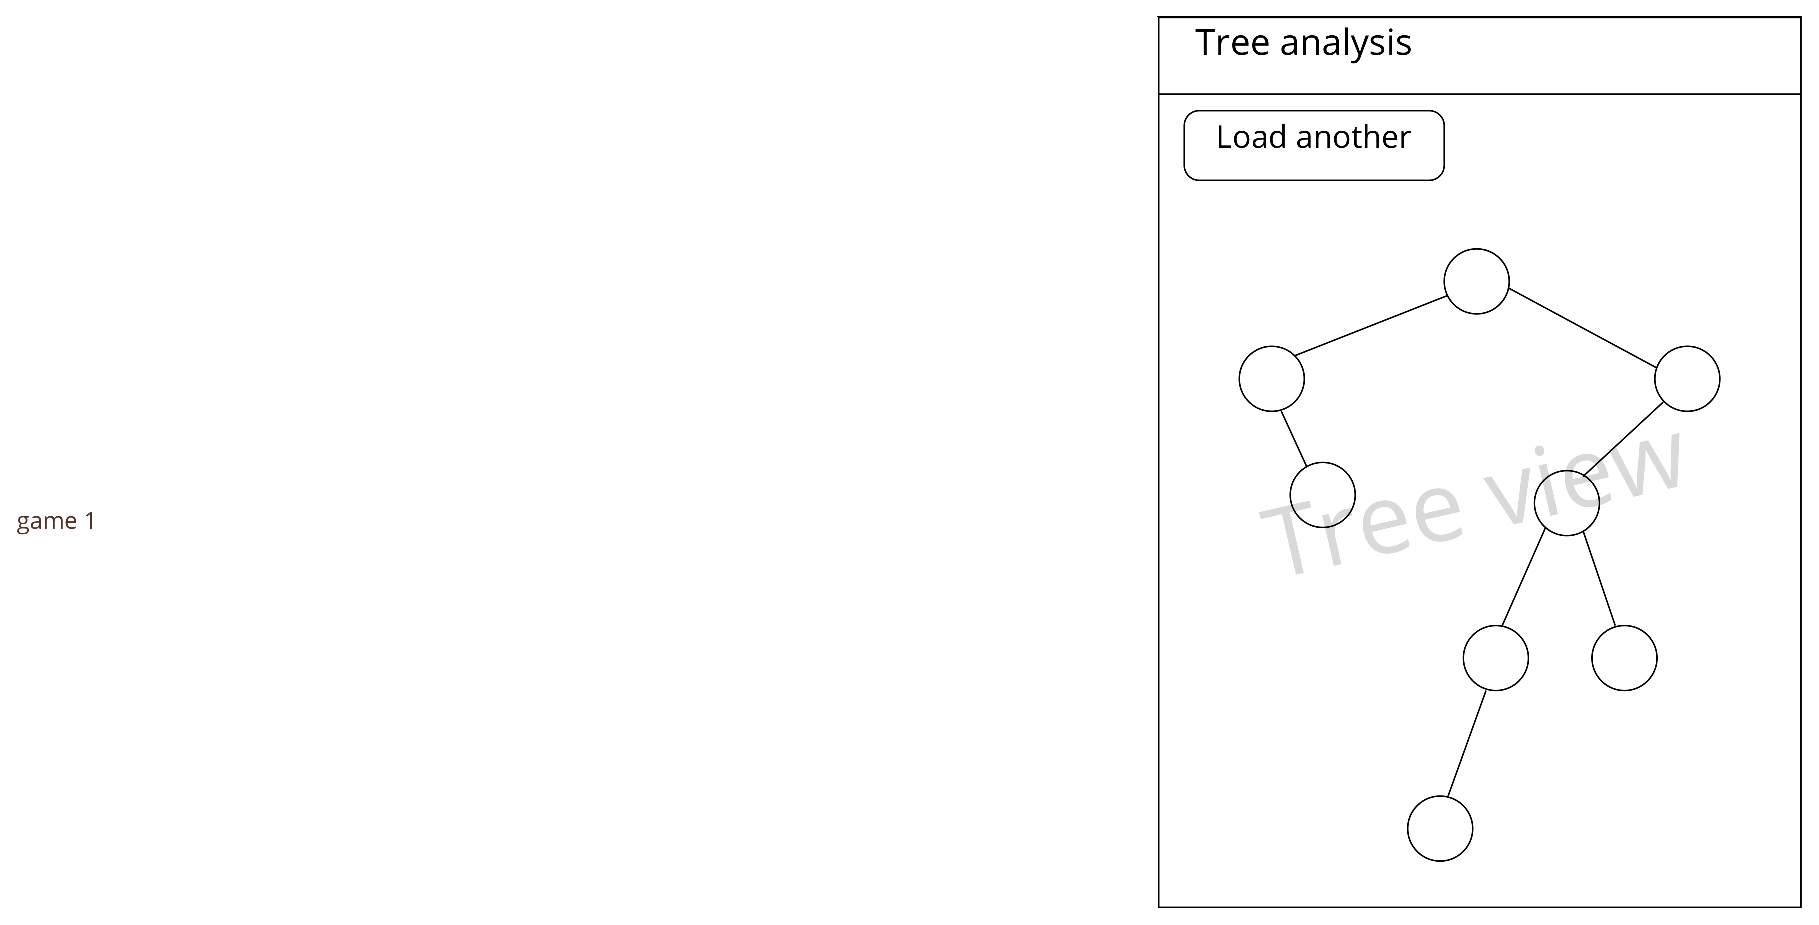
\includegraphics[scale=0.8]{analyze-eps}
		\caption{Okno analizy drzewa}
		\label{rys:analyze_tree}
	\end{figure}
	
	\noindent Kluczową funkcją będzie tutaj możliwość dynamicznego przybliżania i oddalania go wraz z możliwością klikania poszczególnych węzłów w celu pozyskania stanu rozgrywki w danym momencie. Widoczna będzie także informacja o tym, ile razy algorytm odwiedził dany węzeł, ile razy doprowadził on do wygranej oraz średnią nagrodę za ruch w danym węźle.
	
	\clearpage
	
	\subsection{Rozgrywka}
	Poniżej przedstawiony jest przykładowy interfejs graficzny, do którego użytkownik będzie miał dostęp podczas rozgrywki.
	\begin{figure}[h!]
		\centering
		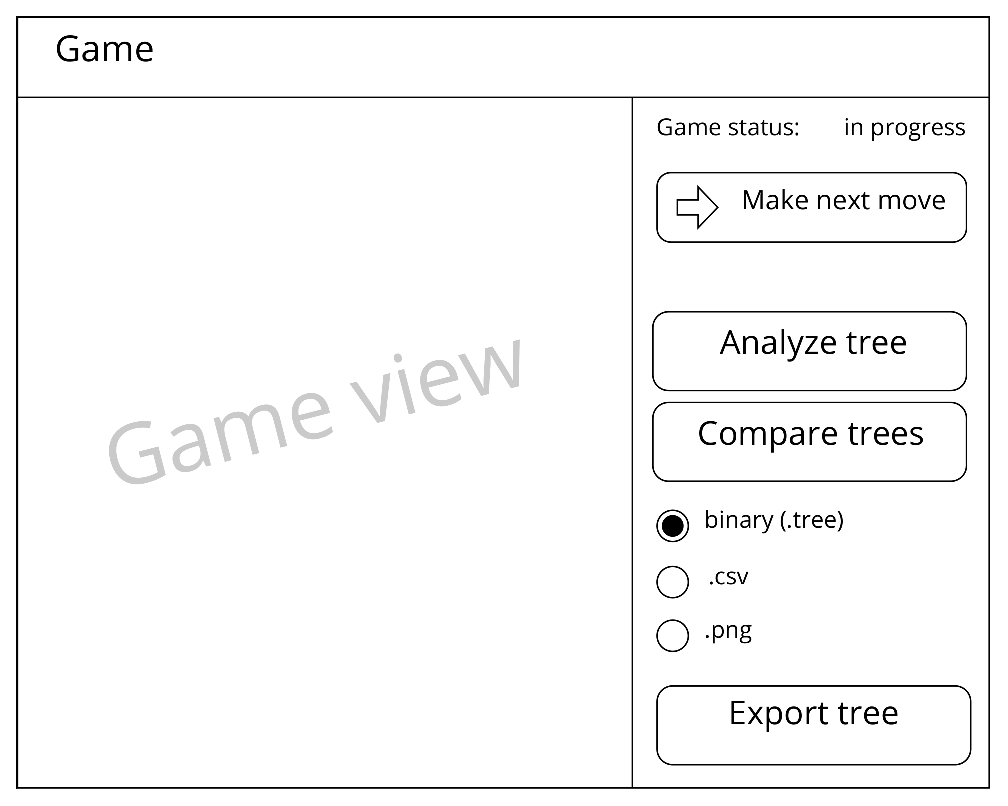
\includegraphics[width=0.7\textwidth]{game-eps}
		\caption{Okno rozgrywki}
		\label{rys:game_view}
	\end{figure}

	\noindent Zgodnie z projektem okna przedstawionym na rysunku \ref{rys:game_view}, widok rozgrywki będzie podzielony na dwie części. Gra zawierać się będzie w wyżej pokazanym oknie po lewej stronie. To tutaj użytkownik za pomocą przygotowanego do gier GUI będzie mógł wykonać ruch. W prawej części okna znajdować się będą opcje związane z aktualnym stanem rozgrywki, między innymi:\\
	
	\begin{itemize}
		\item informacja o aktualnym stanie gry.
		\item wykonaj kolejny ruch - wyłącznie w trybie rozgrywki maszyna kontra maszyna. Użytkownik będzie miał możliwość kontrolowania wykonywanych przez komputer ruchów, aby samemu móc powodować postęp w rozgrywce.
		\item przeanalizuj powstałe drzewo - będzie to przycisk otwierający drugie okno z opisaną już poprzednio analizą drzewa.
		\item porównaj powstałe drzewo z ostatnim - to samo co wyżej, jednak z wyraźnym zaznaczeniem zmian, które zaistniały w nowym drzewie względem starego.
		\item wyeksportuj drzewo do pliku (csv, png lub binarnego).
	\end{itemize}
	
	
	\section{Wybrane technologie}
	Wybraną przez nas technologią do napisania aplikacji, to jest: gier, algorytmu i wizualizacji jest język programowania \textbf{Python} w stabilnej wersji 3.7. Do implementacji gier będziemy posługiwać się biblioteką \textbf{PyGame} (w wersji stabilnej). Wizualizacja będzie wykorzystywać w znacznym stopniu bibliotekę \textbf{VisPy} (OpenGL), w której najbardziej przydatną dla nas funkcją będzie możliwość pisania kodu w języku \textbf{C++} i stosunkowo łatwa integracja z głównym językiem projektu - Pythonem. Wykorzystana przez nas wersja tej biblioteki również będzie wersją stabilną.\\
	
	\noindent Python został przez nas wybrany ze względu na swoją wszechstronność. Posiada on bardzo szeroki zakres bibliotek, co pozwoli nam napisać zdecydowaną większość kodu w jednym języku i przyspieszyć wymianę informacji między komponentami (np. kodem gier a kodem algorytmu MCTS).\\
	
	\noindent VisPy jest nową technologią, która jest wciąż rozwijana, jednak została przez nas wybrana głównie ze względu na:
	\begin{itemize}
		\item współpracę z GPU, co będzie niezbędne podczas wizualizacji setek tysięcy wierzchołków grafu,
		\item obszerną dokumentację.\\
	\end{itemize}

	\noindent Wybór na PyGame padł ze względu na:
	\begin{itemize}
		\item łatwość pisania kodu i przemyślane API,
		\item popularność i dobrą dokumentację.\\
	\end{itemize}	
\end{document}
